Definition \ref{def_interessant} siger, at en region kun bliver taget i
betragtning, hvis den har en masse større end en vis tærskelværdi.
Ved samme fremgangsmåde som i afsnit \ref{region_stoerlse} sammenligner vi fem
forskellige tærskelværdier. Vi kommer frem til, at hvis regionens masse er
under $\frac{1}{4}$ af dens begrænsende rektangel, vil vi ikke tage den med. En
illustration af hvad vi vælger at tage med, kan ses i figur \ref{masse}, hvor
udtrækning af regioner er kørt på billedet \ref{naiv_masse_original}. 
Resultatet kan ses i figur \ref{naiv_masse}.

\begin{figure}[!h]
    \centering
    \subfloat[Original]{
        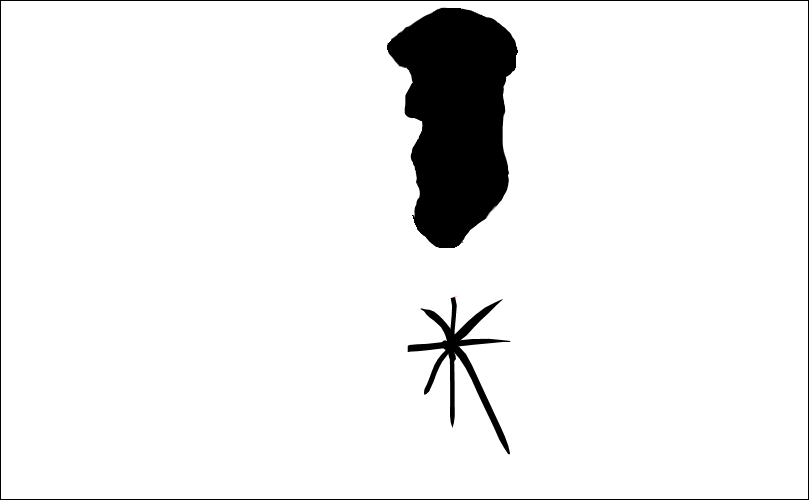
\includegraphics[angle=0,width=0.45\textwidth]{afsnit/afprovning/billeder/naive_losning/mass.png}
        \label{naiv_masse_original}}\hspace{1em}
    \subfloat[To regioner, hvor den ene er sorteret fra på grund af dens masse.]{
        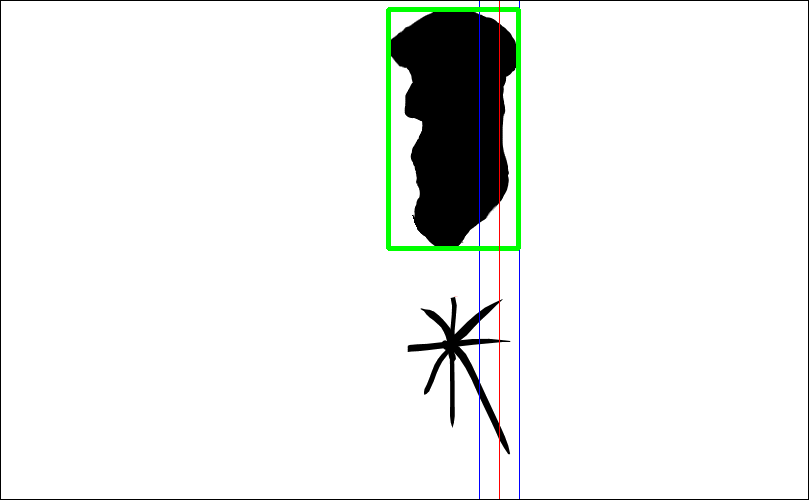
\includegraphics[angle=0,width=0.45\textwidth]{afsnit/afprovning/billeder/naive_losning/naiv_mass.png}
        \label{naiv_masse}}
    \caption{To regioner, som illustrerer forskellen på den region, vi
	tager med, og den, vi ikke tager med.}
	\label{masse}
\end{figure}
